\section{Absolute Latency}
\label{sec:abs_latency}

We defined our latency metric in this paper as relative latency between \ti\
sources, since it is easy to compute and allows consumers to compare feeds
to each other on this aspect. However, it is also critical to know
about the absolute latency distribution of indicators. Absolute latency
represents how fast a feed can actually report a threat, which directly decides
the effectiveness of the data when used in a pro-active way. As we already
discussed in Section~\ref{sec:ip-timing}, absolute latency is hard to measure,
as we do not have ground truth of the underlying threat.

In Section~\ref{sec:completeness}, we used an Internet telescope as our approximation
for ground truth to measure the coverage of scan feeds. In Section~\ref{sec:hash-accuracy},
we used VirusTotal as an oracle to measure the accuracy of file hash feeds.
Although these sources are not real ground truth and it is unclear how far away
they are, these large and well-managed sources can help us, to a certain extent,
profile the performance of \ti\ feeds. In this section, we use these two sources
again to approximate the absolute latency of indicators in scan IP feeds and
malicious file hash feeds.

More specifically, we measure the latency of IPs in scan feeds
relative to the first occurrence time of the same IP in the scanners collected from
the telescope. Considering the massive size of the telescope, it should presumably
detect scanners much sooner after the scanning event actually happened.
We measure latency of file hashes relative to the \texttt{first\_seen} timestamps queried
from VirusTotal. The \texttt{first\_seen} timestamp represents the time when the corresponding
file is first uploaded to VirusTotal. VirusTotal is a very popular service and it is a
convention for many security experts to upload new malware samples to VirusTotal once
they discovered them. Therefore, this timestamp roughly entails when the security
community first noticed the malicious file and can be a good approximation for absolute
latency.

\begin{figure}[t!]
\centering
\subfloat[Latency distribution in scan feeds relative to the Internet telescope]{
	\label{fig:scan_abs_firstseen}
	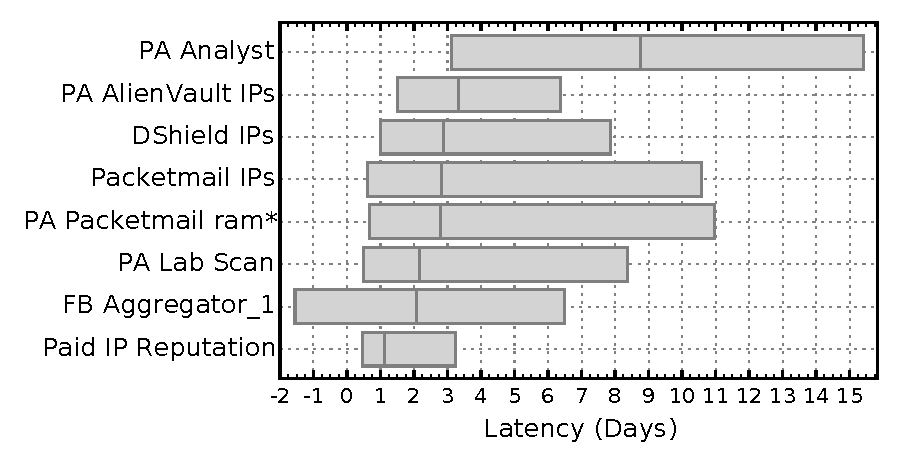
\includegraphics[width=0.8\textwidth]{data_character/images/scan_abs_latency.pdf}}

\subfloat[Latency distribution in file hash feeds relative to VirusTotal]{
	\label{fig:hash_abs_firstseen}
	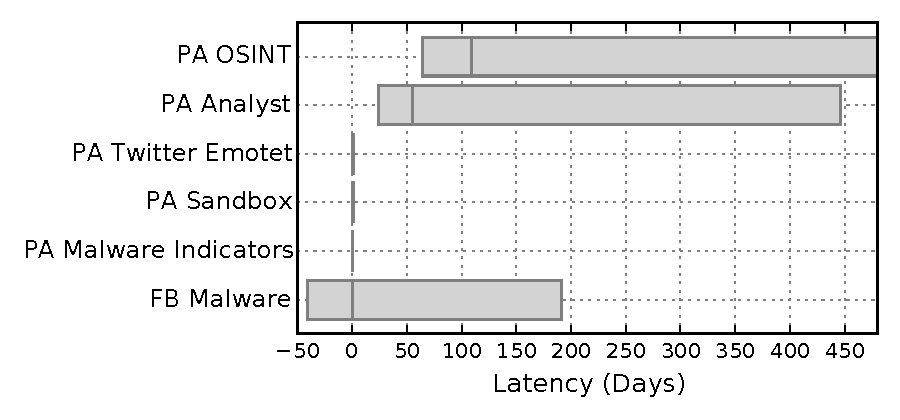
\includegraphics[width=0.8\textwidth]{data_character/images/hash_abs_latency.pdf}}

\caption{Distribution of indicators' latency in scan and file hash feeds.
Note that the scan feeds' distribution are calculated in hour granularity while
the file hash feeds' distribution are calculated in day granularity.}
\label{fig:abs_firstseen}
\end{figure}


Figure~\ref{fig:abs_firstseen} show the latency distribution of each feed, using
the same plotting convention as in Section~\ref{sec:ip-timing}. Some feeds are not
shown in the figure as there are too little data points in those feeds to reason
about distribution.

\finding\
Comparing Figure~\ref{fig:scan_abs_firstseen} to Figure~\ref{fig:scan_firstseen},
we can see that the median latency of feeds are all larger. This is consistent with
our assumption that a large sensor tends to receive indiscriminate scanners sooner.
Scan feeds' median lantecy are one to three days relative to the Internet telescope,
except {\feedTSAnalyst}, whose median latency is almost nine days.
The order of median latency between feeds changed compared with Figure~\ref{fig:scan_firstseen},
but since the original relative median latencies among scan feeds are very close,
the new order here is more likely to be statistics variances. Also, note that
although the {\feedTSAlienVault} seems much slower than it is in
Figure~\ref{fig:scan_firstseen}, its 75 percentile latency is still the second
smallest one.

On the other hand, the latency distributions of hash feeds vary more dramatically.
PA Malware Indicators, PA Sandbox and PA Twitter Emotet are almost as fast as
VirusTotal: all three feeds have 25 percentile and median latency equal to zero.
PA OSINT and PA Analyst are comparatively much slower, and PA OSINT even has a 75
percentile latency of 1680 days. This might be because of the heterogeneous nature of
malware feeds. The figure also shows that feed volumes do not imply
their latency, as PA Analyst and FB Malware are much slower than the small hash
feeds.

Figure~\ref{fig:abs_firstseen} demonstrates that the Internet telescope and VirusTotal
are indeed good approximations for absolute latency measurement, as most
indicators in \ti\ feeds are observed relatively later. However, every scan
feed has over 2\% of its indicators detected earlier than the telescope did.
{\feedFBBasecamp} and {\feeddshield} even have over 10\% of their indicators observed
earlier. There is also a similar case in file hash feeds. This aligns with
our observation in Section~\ref{sec:ip-timing} that small feeds can still report
a non-trivial amount of their data first. Another interesting observation is that
both Facebook feeds, {\feedFBBasecamp} and FB Malware, have a large percent of
their data observed earlier than the telescope or VirusTotal. This again suggests
that Facebook (and its threat intelligence partners) might face more targeted
threats, so those threats will be first observed by Facebook.
